\documentclass{article}
\usepackage[utf8x]{inputenc}
\usepackage{ucs}
\usepackage{amsmath} 
\usepackage{amsfonts}
\usepackage{upgreek}
\usepackage[english,russian]{babel}
\usepackage{graphicx}
\usepackage{float}
\usepackage{textcomp}
\usepackage{hyperref}
\usepackage{geometry}
  \geometry{left=2cm}
  \geometry{right=1.5cm}
  \geometry{top=1cm}
  \geometry{bottom=2cm}
\usepackage{tikz}
\usepackage{ccaption}
\usepackage{multicol}

\usepackage{listings}
%\setlength{\columnsep}{1.5cm}
%\setlength{\columnseprule}{0.2pt}


\begin{document}
\pagenumbering{gobble}

\lstset{
  language=C,                % choose the language of the code
  basicstyle=\linespread{1.1}\ttfamily,
  columns=fixed,
  fontadjust=true,
  basewidth=0.5em,
  keywordstyle=\color{blue}\bfseries,
  commentstyle=\color{gray},
  stringstyle=\ttfamily\color{orange!50!black},
  showstringspaces=false,
  %numbers=false,                   % where to put the line-numbers
  numbersep=5pt,
  numberstyle=\tiny\color{black},
  numberfirstline=true,
  stepnumber=1,                   % the step between two line-numbers.        
  numbersep=10pt,                  % how far the line-numbers are from the code
  backgroundcolor=\color{white},  % choose the background color. You must add \usepackage{color}
  showstringspaces=false,         % underline spaces within strings
  captionpos=b,                   % sets the caption-position to bottom
  breaklines=true,                % sets automatic line breaking
  breakatwhitespace=true,         % sets if automatic breaks should only happen at whitespace
  xleftmargin=.2in,
  extendedchars=\true,
  keepspaces = true,
}
\lstset{literate=%
   *{0}{{{\color{red!20!violet}0}}}1
    {1}{{{\color{red!20!violet}1}}}1
    {2}{{{\color{red!20!violet}2}}}1
    {3}{{{\color{red!20!violet}3}}}1
    {4}{{{\color{red!20!violet}4}}}1
    {5}{{{\color{red!20!violet}5}}}1
    {6}{{{\color{red!20!violet}6}}}1
    {7}{{{\color{red!20!violet}7}}}1
    {8}{{{\color{red!20!violet}8}}}1
    {9}{{{\color{red!20!violet}9}}}1
}

\renewcommand{\thesubsection}{\arabic{subsection}}
\makeatletter
\def\@seccntformat#1{\@ifundefined{#1@cntformat}%
   {\csname the#1\endcsname\quad}%    default
   {\csname #1@cntformat\endcsname}}% enable individual control
\newcommand\section@cntformat{}     % section level 
\newcommand\subsection@cntformat{Задача \thesubsection.\space} % subsection level
\newcommand\subsubsection@cntformat{\thesubsubsection.\space} % subsubsection level
\makeatother


\title{Семинар \#6: Указатели и память. Домашнее задание. \vspace{-5ex}}\date{}\maketitle


\subsection{Создание указателей}
Решения всех подзадач этой части -- одна строка. Результат выполнения задания -- \texttt{.txt} файл, который содержит все эти строки.

\begin{enumerate}
\item В следующей программе создаётся переменная \texttt{a} типа \texttt{int}:
\begin{lstlisting}
int main() 
{
    int a = 1234;
    // Тут нужно написать 1 строку кода
}
\end{lstlisting}
Создайте указатель \texttt{p} и инициализируйте его адресом переменной \texttt{a}.


\item В следующей программе создаётся переменная \texttt{a} типа \texttt{double}:
\begin{lstlisting}
int main() 
{
    double a = 12.34;
    // Тут нужно написать 1 строку кода
}
\end{lstlisting}
Создайте указатель \texttt{p} и инициализируйте его адресом переменной \texttt{a}.

\item В следующей программе создаётся переменная \texttt{a} типа \texttt{char}:
\begin{lstlisting}
int main() 
{
    char a = ')';
    // Тут нужно написать 1 строку кода
}
\end{lstlisting}
Создайте указатель \texttt{p} и инициализируйте его адресом переменной \texttt{a}.

\item В следующей программе создаётся массив \texttt{array} из элементов типа \texttt{int}:
\begin{lstlisting}
int main() 
{
    int array[5] = {10, 20, 30, 40, 50};
    // Тут нужно написать 1 строку кода
}
\end{lstlisting}
Создайте указатель \texttt{p} и сделайте так, чтобы он указывал на первый элемент массива (индекс \texttt{0}).


\item В следующей программе создаётся строка -- массив \texttt{str} из элементов типа \texttt{char}:
\begin{lstlisting}
int main() 
{
    char str[20] = "Sapere Aude";
    // Тут нужно написать 1 строку кода
}
\end{lstlisting}
Создайте указатель \texttt{p} и сделайте так, чтобы он указывал на символ \texttt{'A'}  из строки \texttt{str}.
\end{enumerate}












\subsection{Использование указателей}
Решения всех подзадач этой части -- одна строка. Результат выполнения задания -- \texttt{.txt} файл, который содержит все эти строки.
\begin{enumerate}
\item В следующей программе была создана переменная \texttt{a} и указатель на неё \texttt{p}. Удвойте значение переменной \texttt{a}, используя только указатель \texttt{p}. Нужно использовать указатель \texttt{p}, саму переменную \texttt{a} использовать нельзя.
\begin{multicols}{2}
\begin{lstlisting}
#include <stdio.h>
int main() 
{
    int a = 1234;
    int* p = &a;
    // Тут нужно написать 1 строку кода
    
    printf("%i\n", a);
}
\end{lstlisting}

\vfill \null    
\columnbreak
\vfill \null 

\begin{center}
\vspace{1cm} 
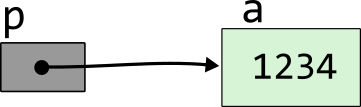
\includegraphics[scale=1]{../images/pointer_schemes/pointer_to_int.png}
\end{center}
\end{multicols}

\item В следующей программе была создана переменная \texttt{a} типа \texttt{float} и указатель на неё \texttt{p}. Возведите значение переменной \texttt{a} в квадрат, используя только указатель \texttt{p}. Нужно использовать только указатель \texttt{p}, саму переменную \texttt{a} использовать нельзя.
\begin{multicols}{2}
\begin{lstlisting}
#include <stdio.h>
int main() 
{
    float a = 1.5;
    float* p = &a;
    // Тут нужно написать 1 строку кода
    
    printf("%f\n", a);
}
\end{lstlisting}

\vfill \null    
\columnbreak
\vfill \null 

\begin{center}
\vspace{1cm} 
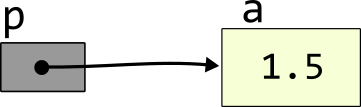
\includegraphics[scale=1]{../images/pointer_schemes/pointer_to_float.png}
\end{center}
\end{multicols}


\item В следующей программе была создана переменная \texttt{a} типа \texttt{char} и указатель на неё \texttt{p}. Переведите символ, хранящийся в переменной \texttt{a} в верхний регистр, используя только указатель \texttt{p}. Нужно использовать только указатель \texttt{p}, саму переменную \texttt{a} использовать нельзя.
\begin{multicols}{2}
\begin{lstlisting}
#include <stdio.h>
int main() 
{
    char a = 't';
    char* p = &a;
    // Тут нужно написать 1 строку кода
    
    printf("%c\n", a);
}
\end{lstlisting}

\vfill \null    
\columnbreak
\vfill \null 

\begin{center}
\vspace{1cm} 
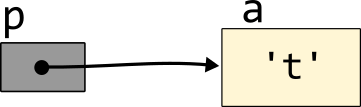
\includegraphics[scale=1]{../images/pointer_schemes/pointer_to_char.png}
\end{center}
\end{multicols}


\newpage
\item В следующей программе был создан массив \texttt{array} переменных  типа \texttt{int} и указатель \texttt{p} на первый элемент массива. 
\begin{multicols}{2}
\begin{lstlisting}
#include <stdio.h>
int main() 
{
    int array[5] = {10, 20, 30, 40, 50};
    int* p = &array[0];

    for (int i = 0; i < 5; ++i) 
        printf("%i ", array[i]);
}
\end{lstlisting}
\vfill \null    
\columnbreak
\vfill \null 
\begin{center}
\vspace{1cm} 
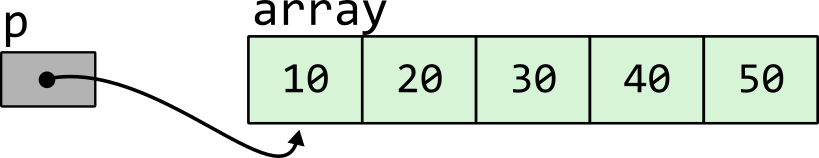
\includegraphics[scale=0.8]{../images/pointer_schemes/pointer_to_int_array.png}
\end{center}
\end{multicols}

\begin{enumerate}
\item Добавьте \texttt{1} к первому элементу массива (\texttt{array[0]}), используя только указатель \texttt{p}. Нужно использовать только указатель \texttt{p}, сам массив \texttt{array} использовать нельзя. Решение -- 1 строка.
\item Добавьте \texttt{1} к четвёртому элементу массива (\texttt{array[3]}), используя только указатель \texttt{p}. Нужно использовать только указатель \texttt{p}, сам массив \texttt{array} использовать нельзя. Менять \texttt{p} тоже нельзя. Решение -- 1 строка.

\item Добавьте \texttt{1} ко всем элементам массива. Нужно использовать только указатель \texttt{p}, сам массив \texttt{array} использовать нельзя. Решение -- 1 цикл.
\end{enumerate}


\item В следующей программе был создан массив \texttt{array} переменных  типа \texttt{int} и указатель \texttt{p} на четвёртый элемент массива (\texttt{array[3]}). 
\begin{multicols}{2}
\begin{lstlisting}
#include <stdio.h>
int main() 
{
    int array[5] = {10, 20, 30, 40, 50};
    int* p = &array[3];
    
    for (int i = 0; i < 5; ++i)
        printf("%i ", array[i]);
}
\end{lstlisting}
\vfill \null    
\columnbreak
\vfill \null 
\begin{center}
\vspace{1cm} 
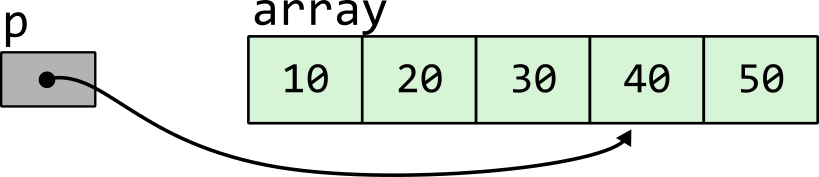
\includegraphics[scale=0.8]{../images/pointer_schemes/pointer_to_int_array_index4.png}
\end{center}
\end{multicols}

\begin{enumerate}
\item Добавьте \texttt{1} к первому элементу массива (\texttt{array[0]}), используя только указатель \texttt{p}. Нужно использовать только указатель \texttt{p}, сам массив \texttt{array} использовать нельзя. Менять \texttt{p} тоже нельзя. Решение -- 1 строка.
\item Добавьте \texttt{1} к пятому элементу массива (\texttt{array[4]}), используя только указатель \texttt{p}. Нужно использовать только указатель \texttt{p}, сам массив \texttt{array} использовать нельзя. Менять \texttt{p} тоже нельзя. Решение -- 1 строка.
\item Добавьте \texttt{1} ко всем элементам массива. Нужно использовать только указатель \texttt{p}, сам массив \texttt{array} использовать нельзя. Решение -- 1 цикл.
\end{enumerate}



\newpage


\item В следующей программе была создана строка \texttt{str} и указатель \texttt{p} на первый символ строки. 
\begin{multicols}{2}
\begin{lstlisting}
#include <stdio.h>
int main() 
{
    char str[] = "sapere aude";
    char* p = &str[0];

    printf("%s\n", str);
}
\end{lstlisting}
\vfill \null    
\columnbreak
\vfill \null 
\begin{center}
\vspace{1cm} 
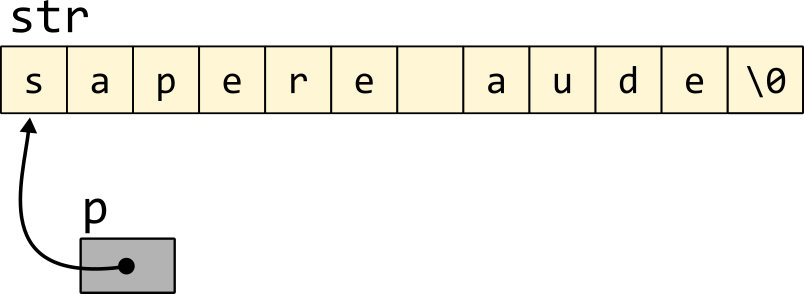
\includegraphics[scale=0.8]{../images/pointer_schemes/pointer_to_char_array.png}
\end{center}
\end{multicols}

\begin{enumerate}
\item Переведите в верхний регистр первую букву строки, используя только указатель \texttt{p}. Нужно использовать только указатель \texttt{p}, саму строку \texttt{str} использовать нельзя. Решение -- 1 строка.
\item Переведите в верхний регистр первую букву второго слова строки, используя только указатель \texttt{p}. Нужно использовать только указатель \texttt{p}, саму строку \texttt{str} использовать нельзя. Решение -- 1 строка.

\item Переведите в верхний регистр все буквы строки, используя только указатель \texttt{p}. Нужно использовать только указатель \texttt{p}, саму строку \texttt{str} использовать нельзя. Решение -- 1 цикл
\end{enumerate}


\item В следующей программе есть переменная \texttt{a} типа \texttt{int}, указатель \texttt{p} на эту переменную и указатель \texttt{q} на \texttt{p}. Удвойте значение переменной \texttt{a}, используя только указатель \texttt{q}. Нужно использовать только указатель \texttt{q}.
\begin{multicols}{2}
\begin{lstlisting}
#include <stdio.h>
int main() 
{
    int a = 1234;
    int* p = &a;
    int** q = &p;
    // Тут нужно написать 1 строку кода
    printf("%i\n", a);
}
\end{lstlisting}

\vfill \null    
\columnbreak
\vfill \null 

\begin{center}
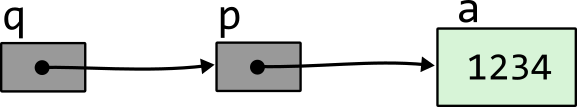
\includegraphics[scale=1]{../images/pointer_schemes/pointer_to_pointer_to_int.png}
\end{center}
\end{multicols}

\end{enumerate}











\newpage
\subsection{Указатель в массиве}
Пусть есть массив и указатель на 4-й элемент этого массива:
\begin{lstlisting}
int numbers[6] = {4, 8, 15, 16, 23, 42};
int* p = &numbers[3];
\end{lstlisting}

\begin{center}
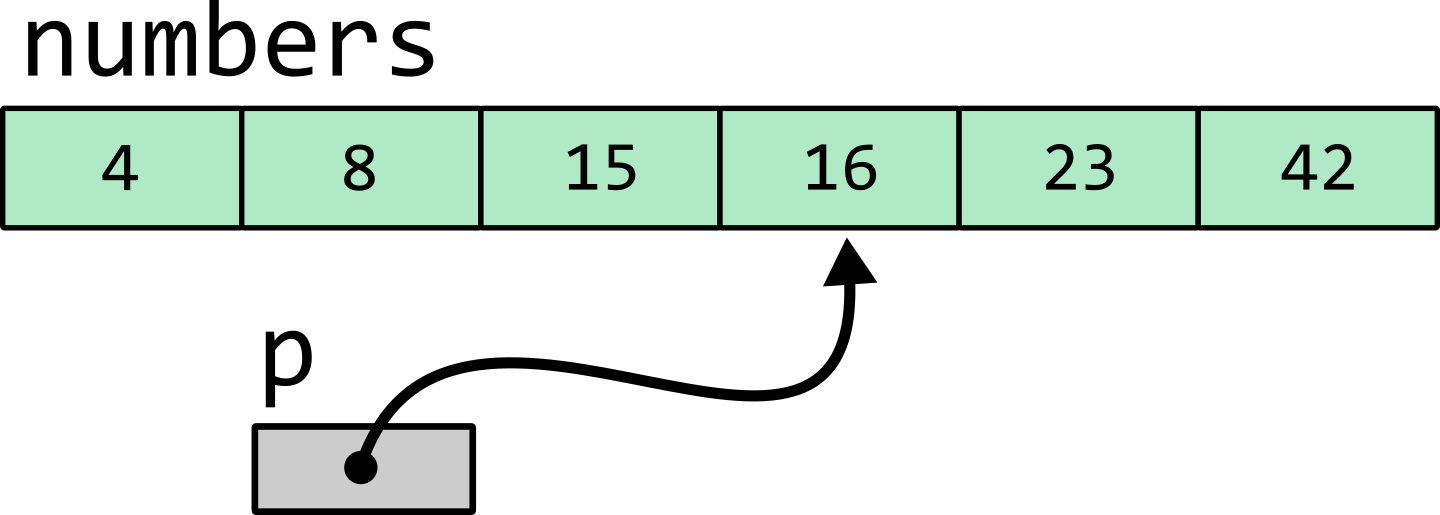
\includegraphics[scale=0.7]{../images/pointer_task_arithmetics.png}
\end{center}

Чему равны следующие выражения:
\begin{multicols}{3}
\begin{enumerate}
\item \begin{verbatim} numbers[5] \end{verbatim}
\item \begin{verbatim} *p \end{verbatim}
\item \begin{verbatim} *(p+1) \end{verbatim}
\item \begin{verbatim} *(p-2) \end{verbatim}
\item \begin{verbatim} p[0] \end{verbatim}
\item \begin{verbatim} p[1] \end{verbatim}
\item \begin{verbatim} p[-2] \end{verbatim}
\item \begin{verbatim} *numbers \end{verbatim}
\item \begin{verbatim} *(numbers+5) \end{verbatim}
\item \begin{verbatim} p - numbers \end{verbatim}
\item \begin{verbatim} (short*)p - (short*)numbers \end{verbatim}
\item \begin{verbatim} (char*)p - (char*)numbers \end{verbatim}
\end{enumerate}
\end{multicols}

Решение этой задачи -- \texttt{.txt} файл со всеми ответами.


\subsection{Куб по указателю}
Напишите функцию \texttt{cube}, которая будет принимать на вход указатель, содержащий адрес некоторой переменной типа \texttt{float}. Функция должна возводиить в куб переменную, чей адрес хранит входящий указатель. Вызовите эту функцию из \texttt{main} и протестируйте её.

\subsection{Умножение массива на 2}
Напишите функцию \texttt{void mult2\_array(int* p, size\_t n)}, которая принимает указатель на первый элемент некоторого массива и число \texttt{n}, равное размеру этого массива. Вам нужно, используя этот указатель, увеличить все элементы массива в 2 раза.


\subsection{Обращение строки}
Напишите функцию \texttt{void reverse\_array(char* s)}, которая принимает указатель на первый элемент некоторой строки обращать эту строку.


\subsection{Квадратное уравнение}
Напишите функцию \texttt{int solve\_quadratic(double a, double b, double c, double* px1, double* px2)}, которая должна решать квадратное уравнение с коэффициентами \texttt{a}, \texttt{b} и \texttt{c}. Результат функция должна записывать по адресам \texttt{px1} и \texttt{px2}. Функция должна возвращать:
\begin{itemize}
\item \texttt{0} - если корней нет. По адресам \texttt{px1} и \texttt{px2} ничего записывать в этом случае не надо.
\item \texttt{1} - если есть один корень. Его нужно записать по адресу \texttt{px1}.
\item \texttt{2} - если есть два корня. Их нужно записать по адресам \texttt{px1} и \texttt{px2}.

Все сравнения делать с точностью $\epsilon = 10^{-10}$ .

\end{itemize}

\subsection{Изменить символы:}
Напишите функцию \texttt{void set\_characters(char* begin, char* end, char c)}, которая задаёт символы в строке символом \texttt{c}. Начиная с символа, на который указывает \texttt{begin} и заканчивая символом на который указывает \texttt{end} (но не включая его). Гарантируется, что \texttt{end} указывает на символ, находящийся в этой же строке и не левее символа, на который указывает \texttt{begin}. Протестируйте функцию с помощью следующего кода:
\begin{lstlisting}
#include <stdio.h>
// Тут нужно написать функции set_characters

int main() 
{
    char s[] = "Sapere Aude";
    set_characters(&s[2], &s[8], 'b');
    printf("%s\n", s); // Должно напечатать Sabbbbbbude
    set_characters(s, &s[4], 'a');
    printf("%s\n", s); // Должно напечатать aaaabbbbude
}
\end{lstlisting}



\newpage
\subsection{Печать разных типов:}
Напишите функцию \texttt{void polyprint(const char* type, void* p)}, которая должна будет печатать то, на что указывает указатель \texttt{p}. Тип того, на что указывает \texttt{p}, задаётся с помощью первой переменной и может принимать следующие значения:
\begin{itemize}
\item Если \texttt{type == "Integer"}, то \texttt{p} указывает на целое число типа \texttt{int}.
\item Если \texttt{type == "Float"}, то \texttt{p} указывает на вещественное число типа \texttt{float}.
\item Если \texttt{type == "Character"}, то \texttt{p} указывает на символ (тип \texttt{char}).
\item Если \texttt{type == "Book"}, то \texttt{p} указывает на структуру \texttt{Book} (определение этой структуры смотрите выше).
\item Если \texttt{type == "String"}, то \texttt{p} указывает на первый символ строки.
\item Если \texttt{type == "IntegerArray 15"}, то \texttt{p} указывает на первый элемент массива размером 15. Элементы этого массива имеют тип \texttt{int}. Нужно распечатать все элементы через пробел. Тут нужно использовать функцию \texttt{sscanf}, для того чтобы распарсить строку \texttt{type}.
\item В ином случае функция должна печатать \texttt{Error!}
\end{itemize}
В любом случае, в конце функция должна печатать символ перехода на новую строку. Для сравнения строк нужно пользоваться функцией \texttt{strcmp}. Протестируйте функцию с помощью следующего кода:

\begin{lstlisting}
#include <stdio.h>
struct book 
{
    char title[50];
    int pages;
    float price;
};
typedef struct book Book;

// Тут нужно написать функцию polyprint

int main() 
{
    int a = 123;
    polyprint("Integer", &a);
    float b = 1.5;
    polyprint("Float", &b);
    char c = 'T';
    polyprint("Character", &c);
    
    Book d = {"War and Peace", 1200, 900.0};
    polyprint("Book", &d);
    
    char e[] = "Sapere Aude";
    polyprint("String", e);
    int f[] = {10, 20, 30, 40, 50};
    polyprint("IngerArray 5", f);
}
\end{lstlisting}


\end{document}